\chapter{Software als Medizinprodukt}

Eine Software kann ein eigenständiges Medizinprodukt, ein Zubehör zu einem Medizinprodukt, ein Teil von einem Medizinprodukt oder gar kein Medizinprodukt sein. Ob eine Software ein Medizinprodukt ist wird in der Zweckbestimmung definiert. Mögliche Anhaltspunkte dass es sich um ein Medizinprodukt handelt: alarmieren, analysieren, berechnen, detektieren, diagnostizieren, interpretieren, konvertieren, messen, steuern, überwachen, verstärken.

Die FDA hat einen Leitfaden für Mobile Applikationen herausgegeben. Dabei zählen folgende Applikationen nicht als Medizinprodukt:
\begin{itemize}
	\item Interaktive anatomische Darstellungen / Videos
	\item \textit{Spiele} zur Simulation von Herzstillstands-Situationen (Training für Ärzte)
	\item Informationen betr. Gluten in Lebensmitteln / Restaurants
	\item App zur Verwendung des Smartphones als Lesehilfe
\end{itemize}
Folgende Applikationen sind möglicherweise ein Medizinprodukt, werden aber von der FDA nicht überwacht:
\begin{itemize}
	\item Apps, die Patienten zu therapeutischen Übungen motivieren
	\item Eingabe: allgemein bekannte Zeichen / Symptome; Output: mögliche Erkrankungen; Empfehlungen einen Arzt aufzusuchen
	\item App ermöglicht dem Patienten eine Person zu alarmieren
	\item App, mit welcher Blutdruckmessungen aufgezeichnet und die zeitliche Entwicklung dargestellt werden kann
\end{itemize}
Diese Applikationen sind Medizinprodukte und im Fokus der FDA:
\begin{itemize}
	\item App, welche mit einem Sensor ein EKG aufnimmt
	\item App, welche Herzgeräusche (oder andere Organe) aufnimmt
	\item App mit Sensor, die Augenbewegung aufnimmt um Gleichgewichtsstörungen zu diagnostizieren
	\item App, welche Testtöne zur Diagnose des Hörvermögens generiert
	\item App, welche Hautveränderungen analysiert
\end{itemize}
Falls es sich bei der Software um ein Medizinprodukt handelt, kann sie in eine der folgenden Sicherheitsklassen eingeteilt werden:
\begin{description}
	\item[Klasse A:] keine Verletzung oder Schädigung der Gesundheit ist möglich
	\item[Klasse B:] keine schwere Verletzung ist möglich
	\item[Klasse C:] Tod oder schwere Verletzung ist möglich
\end{description}
Zudem wird die Software von diversen Normen (z.B. ISO 13485 oder ISO 62304 Detaillierte Anweisungen zur Softwareentwicklung) beeinflusst. Abbildung \ref{fig:software} zeigt den Softwareentwicklungsprozess, wobei nicht alle Prozessschritte bei Software der Klasse A oder B nötig sind.

\begin{figure}
\centering
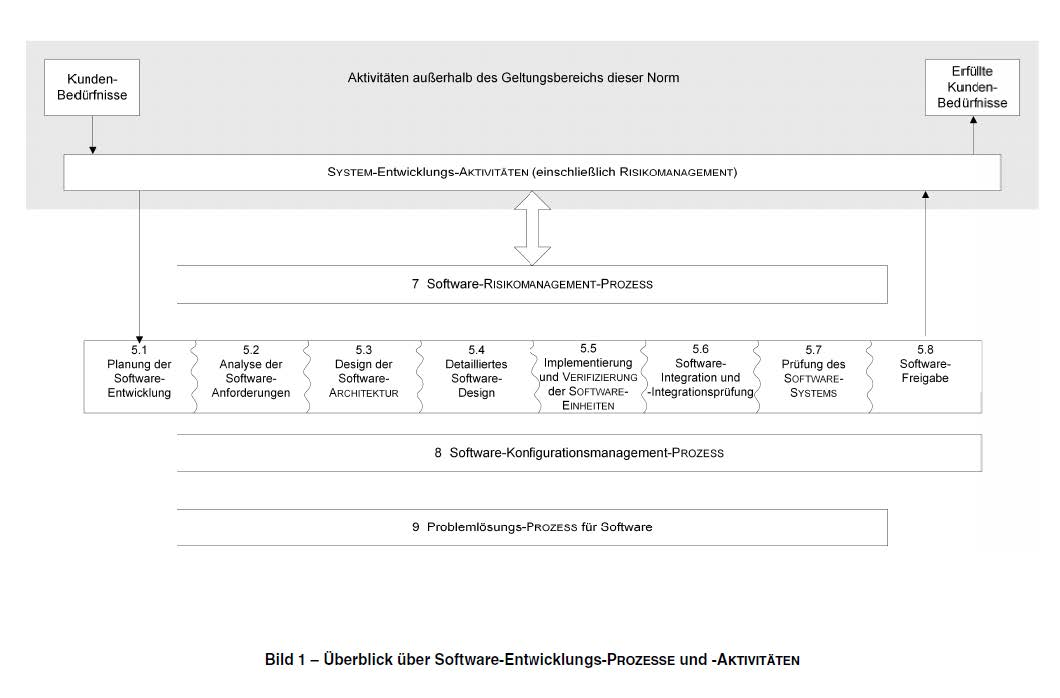
\includegraphics[width=0.7\linewidth]{fig/software}
\caption{Softwareentwicklungsprozess}
\label{fig:software}
\end{figure}
